
\documentclass[../Thesis.tex]{subfiles}
\graphicspath{{\subfix{../figures/}}}
\begin{document}
\chapter{Appendix}

\section{Jordan normal form of infinite matrix sum}\label{app:Jordan normal form of infinite matrix sum}
In this section, we show that for a matrix A with spectral radius less than one, the eigenvalues of $B = \sum_{k=1}^{\infty} A^k$ are exactly $\frac{\lambda_i}{1- \lambda_i}$ for $\lambda_i \in \sigma \left(A\right)$. It is easy to show that if $\left(\lambda, \, v\right)$ is an eigenpair of $B$, then $\left(\frac{\lambda}{1 - \lambda}, v\right)$ is an eigenpair of $B$. However, it is not immediately clear if these are all the eigenpairs of $B$ and hence the eigenvalues. Namely, if the algebraic and geometric multiplicities of the eigenvalues are not the same. To show this, let $J$ be the Jordan normal form of $A$ such that $A$ is similar to $J$ by some invertible matrix $P$. In particular, the Jordan normal form consists of Jordan blocks $J_i$ such that
$$J = \begin{bmatrix}
        J_1 &     &        &     \\
            & J_2 &        &     \\
            &     & \ddots &     \\
            &     &        & J_p
    \end{bmatrix}$$
Hence, $B$ can be written as
\begin{align*}
    B & = \sum_{k=1}^{\infty} A^k  = \sum_{k=1}^{\infty} P^{-1} J^k P  = P^{-1} \sum_{k=1}^{\infty} J^k P
\end{align*}
Note that $J^k$ is given by
$$J^k = \begin{bmatrix}
        J_1^k &       &        &       \\
              & J_2^k &        &       \\
              &       & \ddots &       \\
              &       &        & J_p^k
    \end{bmatrix}$$
Focusing on a single Jordan block $J_i$ given by
$$J_i = \begin{bmatrix}
        \lambda_i & 1         &        &           \\
                  & \lambda_i & 1      &           \\
                  &           & \ddots &           \\
                  &           &        & \lambda_i
    \end{bmatrix},$$
we see that $J_i^k = \lambda_i^k I + T$ where $T$ is a strictly upper-triangular matrix. From this, we see that $\sum_{k = 1}^{\infty} J_i^k = \frac{\lambda_i}{1 - \lambda_i} I + T'$ where $T'$ is another strictly upper-triangular matrix. Thus, $\sum_{k = 1}^{\infty} J_i^k$ has $\frac{\lambda_i}{1 - \lambda_i}$ as diagonal elements, hence there exists some invertible matrix $P_i$ such that $ \sum_{k = 1}^{\infty} J_i^k = \left(P_i\right)^{-1} J_i'  P_i$ where $J_i'$ is a Jordan normal form (with $\frac{\lambda_i}{1 - \lambda_i}$ as diagonal elements) of $\sum_{k = 1}^{\infty} J_i^k$. Combining the above, we have that
\begin{align*}
    \sum_{k=1}^{\infty} J^k &= \begin{bmatrix}
        \sum_{k = 1}^{\infty} J_1^k & & & \\
        & \sum_{k = 1}^{\infty} J_2^k & & \\
        & & \ddots & \\
        & & & \sum_{k= 1}^{\infty} J_p^k
    \end{bmatrix}\\
    & =  \begin{bmatrix}
        P_1^{-1} J_1' P_1 & & & \\
        & P_2^{-1} J_2' P_2 & & \\
        & & \ddots & \\
        & & & P_p^{-1} J_p' P_p
    \end{bmatrix}\\
    & = \begin{bmatrix}
        P_1 & & & \\
        & P_2 & & \\
        & & \ddots & \\
        & & & P_p
    \end{bmatrix}^{-1}
    \begin{bmatrix}
        J_1' & & & \\
        & J_2' & & \\
        & & \ddots & \\
        & & & J_p'
    \end{bmatrix}
    \begin{bmatrix}
        P_1 & & & \\
        & P_2 & & \\
        & & \ddots & \\
        & & & P_p
    \end{bmatrix}
\end{align*}
Let $P'$ be the above block diagonal matrix, consisting of $P_i$s and $J'$ be the block diagonal matrix consisting of $J_i'$s and hence also a Jordan normal form. Then, we can finally write $B$ as
$$B = \left(P' P\right)^{-1} J' P' P$$
In particular, $B$ is similar to the Jordan normal form $J'$ with diagonal elements $\frac{\lambda_i}{1-\lambda_i}$. In particular, the spectrum of $B$ is exactly the elements of the spectrum of $A$ mapped by $\lambda \mapsto \frac{\lambda}{1 - \lambda}$.

\newpage

\section{Pharmaceutical duration and level changes plots}
\begin{figure}[H]
    \centering
    \includegraphics[width = \linewidth]{figures/Multiple cycles data/time vs time scatter.png}
    \caption{}
    \label{fig:time vs time all}
\end{figure}

\begin{figure}[H]
    \centering
    \includegraphics[width = \linewidth]{figures/Multiple cycles data/delta filling vs time scatter.png}
    \caption{}
    \label{fig:time vs level all}
\end{figure}

\begin{figure}[H]
    \centering
    \includegraphics[width = \linewidth]{figures/Multiple cycles data/delta fill vs delta fill scatter.png}
    \caption{}
    \label{fig:level vs level all}
\end{figure}

\newpage

\section{Cleaning operations plots}
\begin{figure}[H]
    \centering
    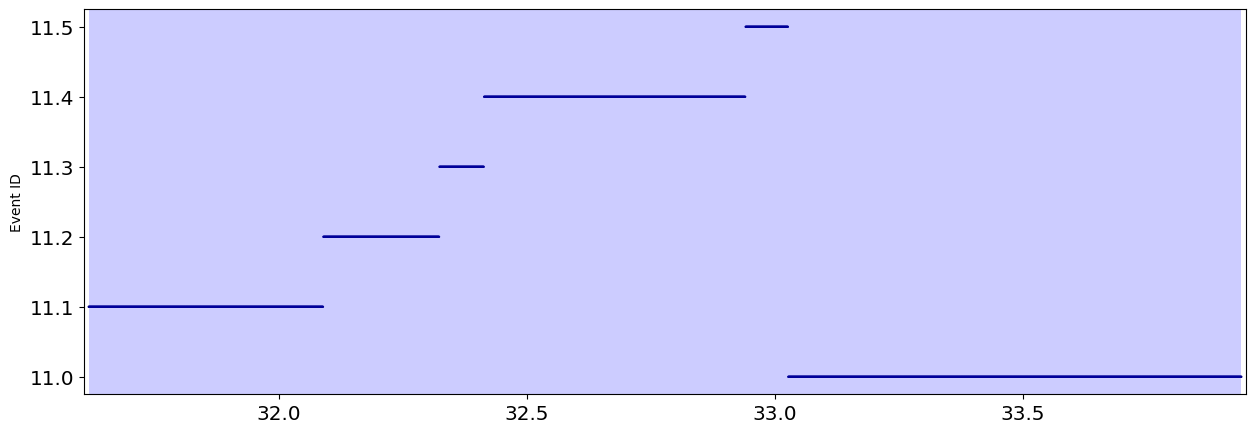
\includegraphics[width=0.9\linewidth]{figures/Multiple cycles data/Cleaning batches timeseries single.png}
    \caption{A single blue rectangle zoomed in}
    \label{fig:cycle cleaning time series single}
\end{figure}

\newpage
\begin{figure}[H]
    \centering
    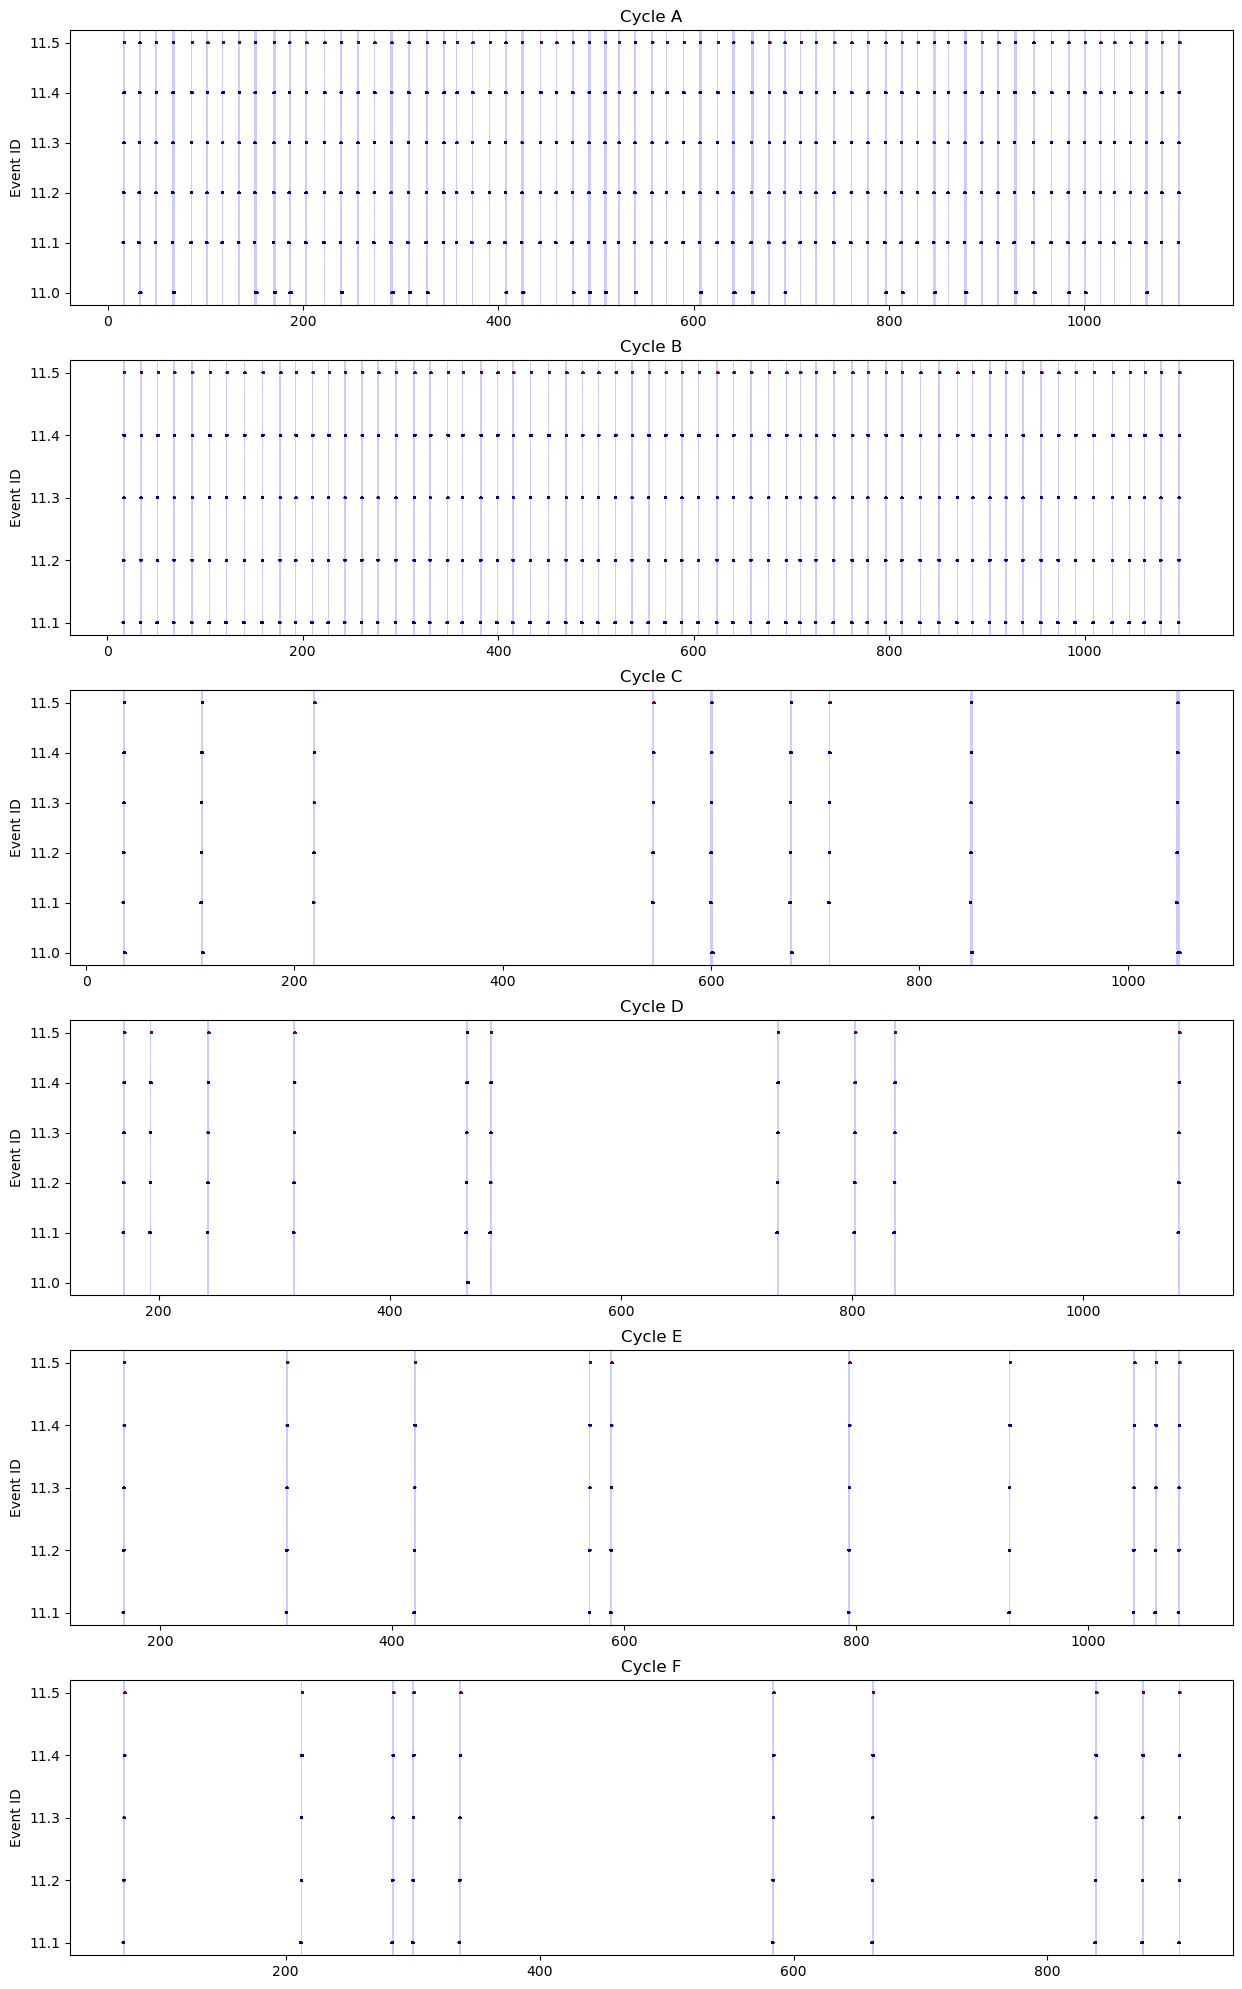
\includegraphics[width=0.9\linewidth]{figures/Multiple cycles data/Cleaning batches.png}
    \caption{Each of the 6 cycles, cleaning (corresponding to \texttt{BatchID = 0} in the time series dataset). Each \textit(Cleaning Procedure), CIP, is highlighted with an opaque interval (the blue rectangles). The dots marked with red (only ID 11.5, but not all of these are red), is if the Cleaning ID is 0.}
    \label{fig:cycle cleaning time series}
\end{figure}


\section{Suicide data}
\begin{table}[H]
    \centering
    \begin{tabular}{cccccc}
        1  & 25 & 40 & 83  & 123 & 256 \\
        1  & 27 & 49 & 84  & 126 & 257 \\
        1  & 27 & 49 & 84  & 129 & 311 \\
        5  & 30 & 54 & 84  & 134 & 314 \\
        7  & 30 & 56 & 90  & 144 & 322 \\
        8  & 31 & 56 & 91  & 147 & 369 \\
        8  & 31 & 62 & 92  & 153 & 415 \\
        13 & 32 & 63 & 93  & 163 & 573 \\
        14 & 34 & 65 & 93  & 167 & 609 \\
        14 & 35 & 65 & 103 & 175 & 640 \\
        17 & 36 & 67 & 103 & 228 & 737 \\
        18 & 37 & 75 & 111 & 231       \\
        21 & 38 & 76 & 112 & 235       \\
        21 & 39 & 79 & 119 & 242       \\
        22 & 39 & 82 & 122 & 256
    \end{tabular}
    \caption{The length of treatment of control patients in suicide study. The data originates from the Mental Health Enquiry (MHE) of England of Wales and was published in 1967.}
    \label{tab:suicide data}
\end{table}

\newpage


\subsection{A better spline}\label{sec:A family of better splines for Copula entropy estimation}
In theory, we could make a set of splines ourselves, that has both of the desired properties of B-splines and M-splines. I.e. a set of piecewise polynomials, which we shall denote $Q_{i,p}$, that has both the property that
$$\sum_{i = 1}^n Q_{i,p} (t) = 1$$
and
$$\int_{0}^{1} Q_{i,p} (t) \, dt = \frac{1}{n} $$
Actually, both M- and B-splines satisfies this for $p = 0$ as they are then both piecewise constant and non-zero on disjoint intervals. From this, one can the construct such sets of $Q_{i,p}$ in the following way. Namely, start with the piecewise constant functions, $Q_{i,0}$ depicted in \autoref{fig:spline order 0 - Q} as boxes in the case $n = 5$.


\begin{figure}[h]
    \centering
    \includesvg[width=.7\linewidth]{figures/MI estimation/Q_spline_construction_step_1.svg}
    \caption{}
    \label{fig:spline order 0 - Q}
\end{figure}

A better spline

\begin{figure}[h]
    \centering
    \includesvg[width=.7\linewidth]{figures/MI estimation/Q-spline construction - step 2.svg}
    \caption{}
    \label{fig:spline order 0 - Q - step 2}
\end{figure}

Cut off function has derivative 0 at top and is halfway down at the sides
\begin{figure}[h]
    \centering
    \begin{subfigure}[t]{0.49\textwidth}
        \centering
        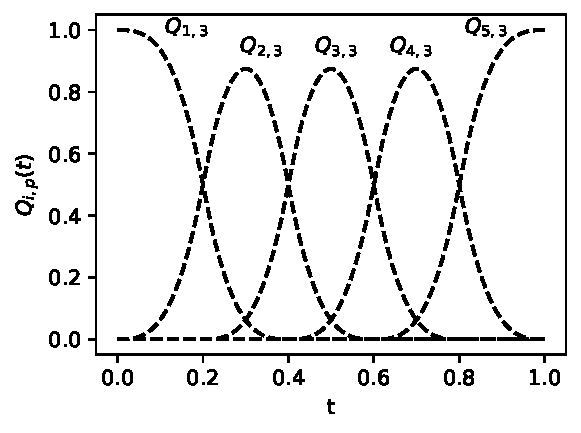
\includegraphics[width=\linewidth]{figures/MI estimation/Q-spline basis functions - degree 3.pdf}
        \caption{}
    \end{subfigure}
    \hfill
    \begin{subfigure}[t]{0.49\textwidth}
        \centering
        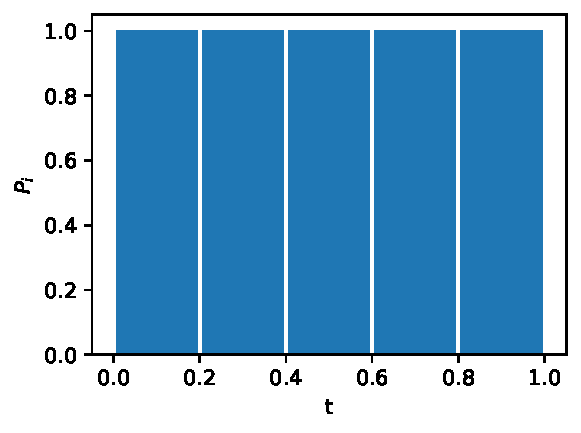
\includegraphics[width=\linewidth]{figures/MI estimation/Q-spline marginal dist - degree 3.pdf}
        \caption{}
    \end{subfigure}
    \caption{$P_i$ is area of each rectangle i.e. $0.2$.}
\end{figure}

\begin{figure}[h]
    \centering
    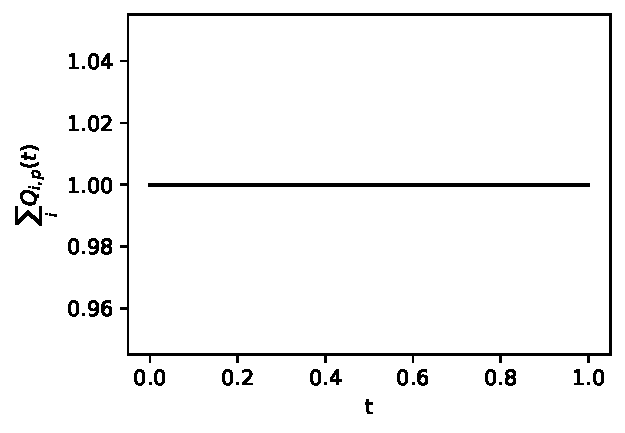
\includegraphics[width = .55\linewidth]{figures/MI estimation/Q-spline coefficient sum - degree 3.pdf}
    \caption{}
    % \label{}
\end{figure}
This example does however not work well for many bins, in particular, due to the splines not overlapping that much i.e. a poor regularization on the smoothness. However, the method used for constructing this set of splines can be extended to bleed into multiple neighboring bins just as for B- and M-splines.

\newpage
\section{M-spline based MI estimation}
\begin{figure}[H]
    \centering
    \begin{subfigure}[t]{0.32\textwidth}
        \centering
        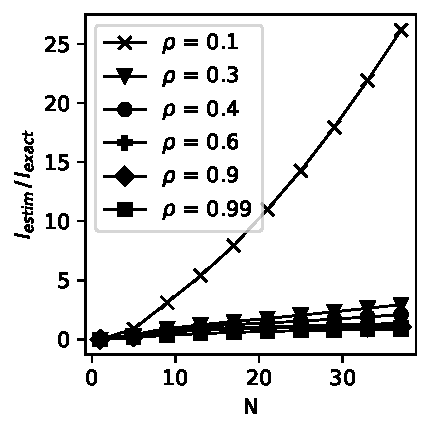
\includegraphics[width=\linewidth]{figures/ND examples/MI calc/gaussian example original all - M-spline - relative error.pdf}
        \caption{}
        % \label{subfig:d}
    \end{subfigure}%
    ~
    \begin{subfigure}[t]{0.32\textwidth}
        \centering
        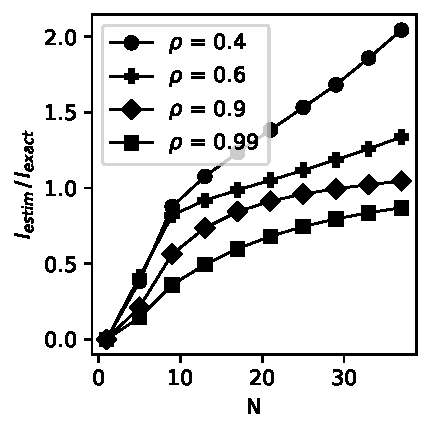
\includegraphics[width=\linewidth]{figures/ND examples/MI calc/gaussian example original zoom - M-spline - relative error.pdf}
        \caption{}
        % \label{subfig:dd}
    \end{subfigure}%
    ~
    \begin{subfigure}[t]{0.32\textwidth}
        \centering
        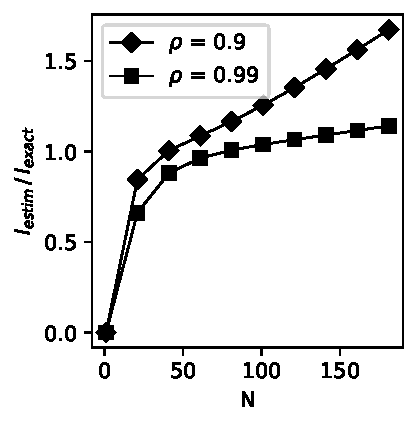
\includegraphics[width=\linewidth]{figures/ND examples/MI calc/gaussian example original high corr - M-spline - relative error.pdf}
        \caption{}
        % \label{subfig:ddd}
    \end{subfigure}
    \caption{}
    \label{fig:M-spline approach results MI - relative error}
\end{figure}

\begin{figure}[H]
    \centering
    \begin{subfigure}[t]{0.4\textwidth}
        \centering
        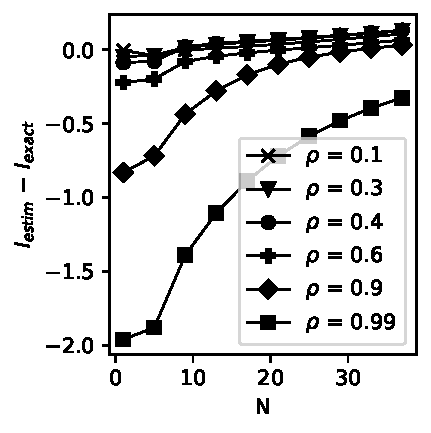
\includegraphics[width=\linewidth]{figures/ND examples/MI calc/gaussian example original zoom - M-spline - error.pdf}
        \caption{}
        % \label{subfig:new MI method all}
    \end{subfigure}%
    ~
    \begin{subfigure}[t]{0.4\textwidth}
        \centering
        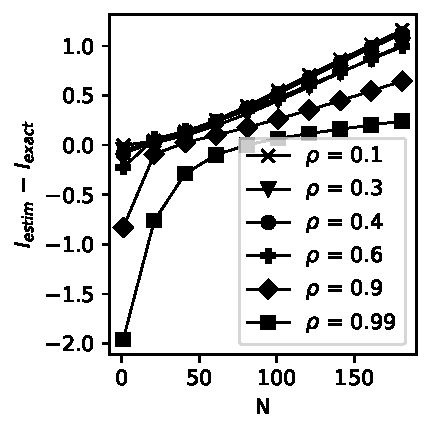
\includegraphics[width=\linewidth]{figures/ND examples/MI calc/gaussian example original all - M-spline - error.pdf}
        \caption{}
        % \label{subfig:new MI method all zoom}
    \end{subfigure}
    \caption{}
    \label{fig:M-spline approach results MI - error}
\end{figure}


\newpage
\section{Confidence interval for absolute correlation in bivariate Gaussian}\label{sec:bivar gauss abs correlation CI}
From \cite{Confidence_in_Correlation}, given a bivariate Gaussian, the confidence distribution of $\rho$ given the empirical correlation $r$ based on $n$ observations is given by
$$f\left(\rho \mid r,\nu\right) = \frac{\nu (\nu-1) \Gamma(\nu-1)}{\sqrt{2\pi} \Gamma(\nu + \frac{1}{2})} \frac{\left(1-r^2\right)^{\frac{\nu-1}{2}} \left(1-\rho^2\right)^{\frac{\nu-2}{2}} }{\left(1-r\rho\right)^{\frac{2\nu-1}{2}}} F\left(\frac{3}{2}, -\frac{1}{2}, \nu+\frac{1}{2}, \frac{1+r\rho}{2}\right)$$
where $F\left(a,b,c,z\right)$ is the Gaussian hypergeometric function and $\nu = n-1$. That is, given a sample correlation $r$, what is the confidence in $\rho$ in terms of a distribution. In the following figure, a sample correlation $r=0.8$ and $r=0$ has been used with varying number of observations (degrees of freedom) in figures \autoref{subfig:gaussian correlation dist 0.8} and \autoref{subfig:gaussian correlation dist 0} respectively.
\begin{figure}[h]
    \centering
    \begin{subfigure}[t]{0.49\linewidth}
        \centering
        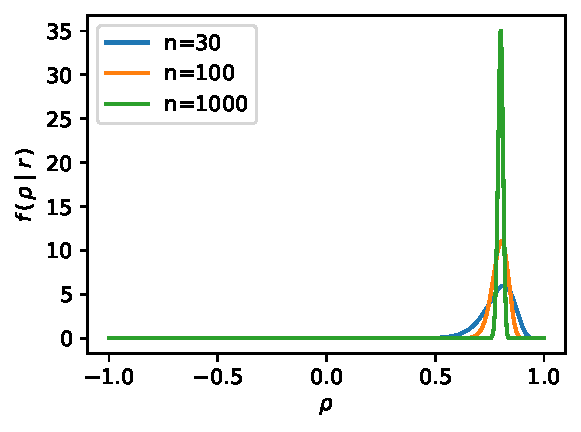
\includegraphics[width=\linewidth]{figures/Gaussian correlation confidence dist/density comparison r 0.8.pdf}
        \caption{}
        \label{subfig:gaussian correlation dist 0.8}
    \end{subfigure}%
    ~
    \begin{subfigure}[t]{0.49\linewidth}
        \centering
        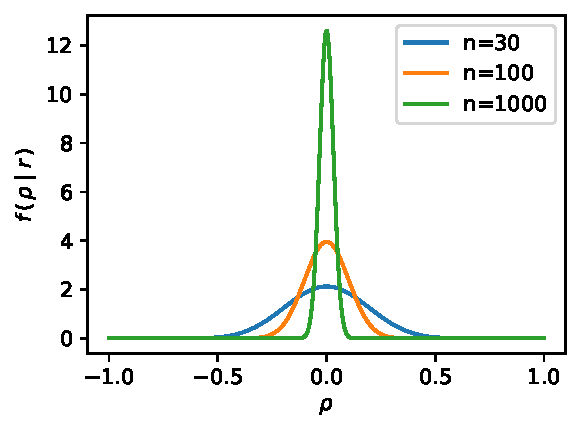
\includegraphics[width=\linewidth]{figures/Gaussian correlation confidence dist/density comparison r 0.pdf}
        \caption{}
        \label{subfig:gaussian correlation dist 0}
    \end{subfigure}
    \caption{$f\left(\rho \mid r, \nu\right)$ shown for $r=0.8$ and $r=0$ in (a) and (b) with $n\in \{30,100,1000\}$. As one would expect, the power i.e. the width of the peak decreases with increasing n and for correlations closer to $0$, the width is the largest.}
\end{figure}
A key property is that $f$ is \textit{even symmetric} in $\rho,\, r$. That is $f(\rho \mid r) = f(-\rho \mid -r)$. Thus, a confidence interval for $\rho$ given $r$ is the negative of the confidence interval given $-r$. In particular, if we only observe $|r|$, we can calculate a confidence interval for $\rho$ up to the sign of the bounds of the interval. Furthermore, as we want a CI for $|\rho|$, it does not matter if $r$ is negative or positive. Hence, without loss of generality, we assume that $r \geq 0$. At this point, to construct a confidence interval for $|\rho|$ we list the following desired properties. Firstly, it should be an exact confidence interval, meaning that for a given significance level $\alpha$, the CI includes the true value exactly $1-\alpha$ fraction of the times. Secondly, if for a given $r$, it can not be rejected that $\rho$ is 0, 0 should also be contained in the interval. Finally, if we reject that $\rho = 0$, we shall have $\alpha/2$ probability mass above and below the bounds of the interval. The above is enough to uniquely define a confidence interval in all cases. Before continuing with how this CI is calculated, we mention that as $r$ is an unbiased estimator of $\rho$, we would preferably want $|r| \in CI_{1-\alpha}\left(|\rho|\right)$ (where $CI_{1-\alpha}\left(|\rho|\right)$ denotes the $1-\alpha$ confidence interval for $|\rho|$). However, although this will in almost every scenario be the case, we can not be sure of this from the above properties and in fact examples with large $\alpha$ can be constructed such that $|r|$ lies just outside the constructed CI.

First, to conform with the second desired property, if it can not be rejected that $\rho = 0$ on a significance level $\alpha$, we will initially compute a CI for $\rho$ (not $|\rho|$) based on $r$ (WLOG chosen to be non-negative). This CI will just be a symmetric CI in the sense that $\alpha/2$ of the probability mass will lie below the lower bound of the CI and above the upper bound of the CI respectively. If $0$ is contained in this CI, we can not reject that $\rho=0$ and vice versa on an $\alpha$ significance level. Thus, if $0$ is contained in this initial CI for $\rho$, we will start the CI for $|\rho|$ at $0$ and determine and upper bound $b$ such that $\alpha$ probability mass is above this $b$. Otherwise, we shall find $a$ and $b$ such that $\alpha/2$ probability mass is below $a$ and above $b$ respectively. Choosing $a$ and $b$ this way also conforms with the third property. Finally, to ensure that the CI contains exactly $1-\alpha$, we define $\tilde{f}$ as the reflected $f$ in $\rho$ such that
$$\tilde{f}\left(\rho_a \mid r_a, \nu\right) = f(\rho_a \mid r_a, \nu) + f(-\rho_a \mid r_a, \nu),\quad \rho_a,r \in [0,1]$$
where $\rho_a$ and $r_a$ is the absolute correlation and empirical correlation respectively. With this $\tilde{f}$, the density at $\rho_a$ is both the density for the negative and positive correlation ensuring that the $\tilde{f}$ has probability mass $1$. Thus, if $a=0$ (i.e. the CI must contain $0$), we find $b$ as the $1-\alpha$ percentile of $\tilde{f}$ and if $a\neq 0$, we take $a$ as the $\alpha/2$ percentile and $b$ as the $1-\alpha/2$ percentile of $\tilde{f}$.

As an example, suppose $r_a=0.06$ with $1000$ observations. Then a $95\%$ CI for $|\rho|$ is $[0, 0.11164]$ whereas if on had observed $r_a = 0.07$ the CI would be $[0.01071, 0.1314]$. These CI could then be used to test the absolute correlation of a bivariate Gaussian i.e. for $r_a = 0.07$ based on $1000$ observations would be rejected as stemming from a Gaussian with absolute correlation $0.01$ on a $5\%$ significance level.


\newpage
\section{Gaussian chain deconvolution}

\begin{figure}[H]
    \centering
    \begin{subfigure}[t]{0.49\textwidth}
        \centering
        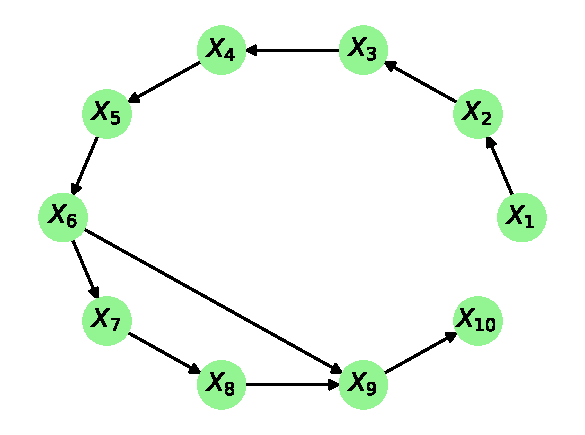
\includegraphics[width=.95\linewidth]{figures/Gaussian Chain Theoretical/Chain graph from triangular G obs - MI - cutoff 2e-2.pdf}
        \caption{}
        % \label{fig:Gaussian 3x3 large s}
    \end{subfigure}
    \hfill
    \begin{subfigure}[t]{0.49\textwidth}
        \centering
        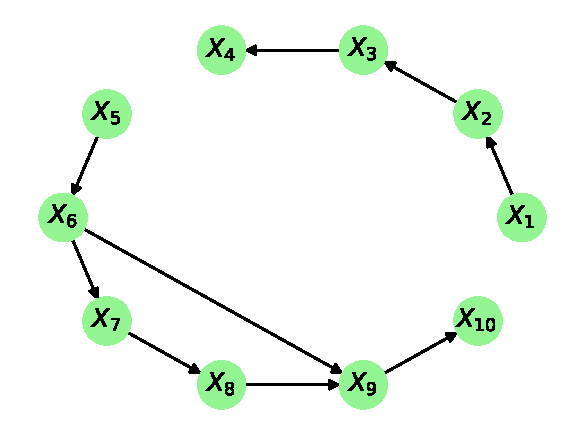
\includegraphics[width=.95\linewidth]{figures/Gaussian Chain Theoretical/Chain graph from triangular G obs - MI - cutoff 2_1e-2.pdf}
        \caption{}
        % \label{fig:Gaussian 3x3 large s}
    \end{subfigure}
    \\[\baselineskip]
    \begin{subfigure}[t]{0.49\textwidth}
        \centering
        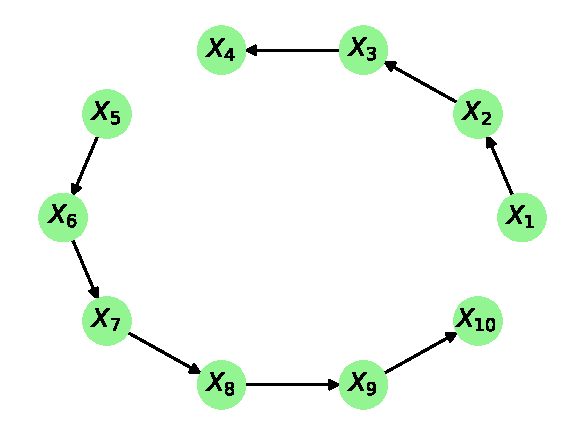
\includegraphics[width=.95\linewidth]{figures/Gaussian Chain Theoretical/Chain graph from triangular G obs - MI - cutoff 4_51e-2.pdf}
        \caption{}
        % \label{fig:Gaussian 3x3 large s}
    \end{subfigure}
    \caption{Triangular, mutual information, cutoff $2\cdot 10^{-10}$, $2.1 \cdot 10^{-2}$ and $4.51 \cdot 10^{-2}$.}
    \label{fig:Gaussian chain symmetric G_obs using mutual information different cutoff}
\end{figure}

\newpage
\begin{figure}
    \centering
    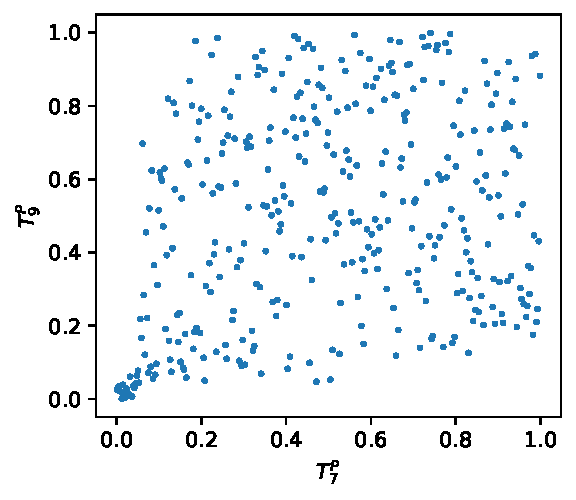
\includegraphics[width=.5\linewidth]{figures/Cycle data/G_dir times - symmetric - TP9 vs TP7.pdf}
    \caption{}
    \label{fig:G_dir times - TP9 vs TP7}
\end{figure}


\newpage
\section{Gaussian network deconvolution}
\begin{figure}[H]
    \centering
    \begin{subfigure}[t]{0.49\textwidth}
        \centering
        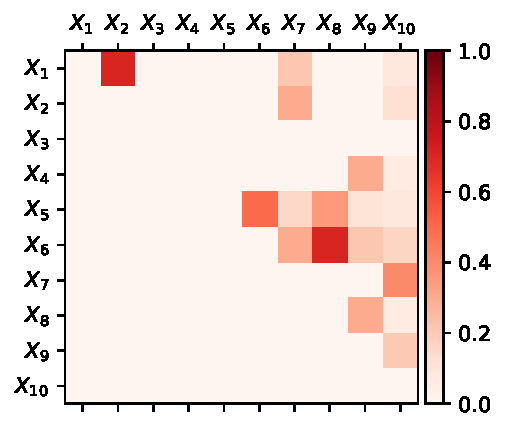
\includegraphics[width=.95\linewidth]{figures/Gaussian Network Theoretical/triangular G obs - cor.pdf}
        \caption{$G_{obs}$}
        % \label{fig:Gaussian 3x3 large s}
    \end{subfigure}
    \hfill
    \begin{subfigure}[t]{0.49\textwidth}
        \centering
        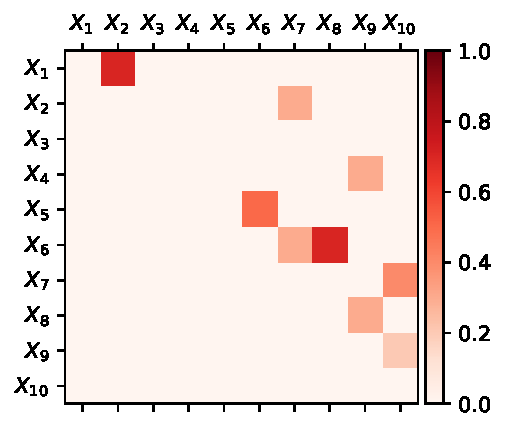
\includegraphics[width=.95\linewidth]{figures/Gaussian Network Theoretical/G dir from triangular G obs - cor.pdf}
        \caption{$G_{dir}$}
        % \label{fig:Gaussian 3x3 large s}
    \end{subfigure}
    \\[\baselineskip]
    \begin{subfigure}[t]{0.49\textwidth}
        \centering
        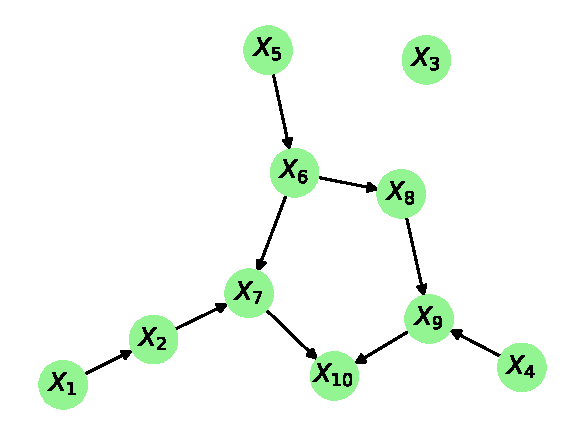
\includegraphics[width=.9\linewidth]{figures/Gaussian Network Theoretical/Graph from triangular G obs - cor.pdf}
        \caption{$G_{dir}$ as a graph}
        % \label{fig:Gaussian 3x3 large s}
    \end{subfigure}
    \caption{For the linear network defined in \autoref{eq:example Gaussian network}, using a triangular $G_{obs}$ (a) with the true topological structure we are able to perfectly rediscover the causal structure as seen in (b) and (c).}
    \label{fig:Gaussian network triangular G_obs using correlation}
\end{figure}

\newpage
\section{Pharmaceutical process deconvolution}
\begin{figure}[ht]
    \centering
    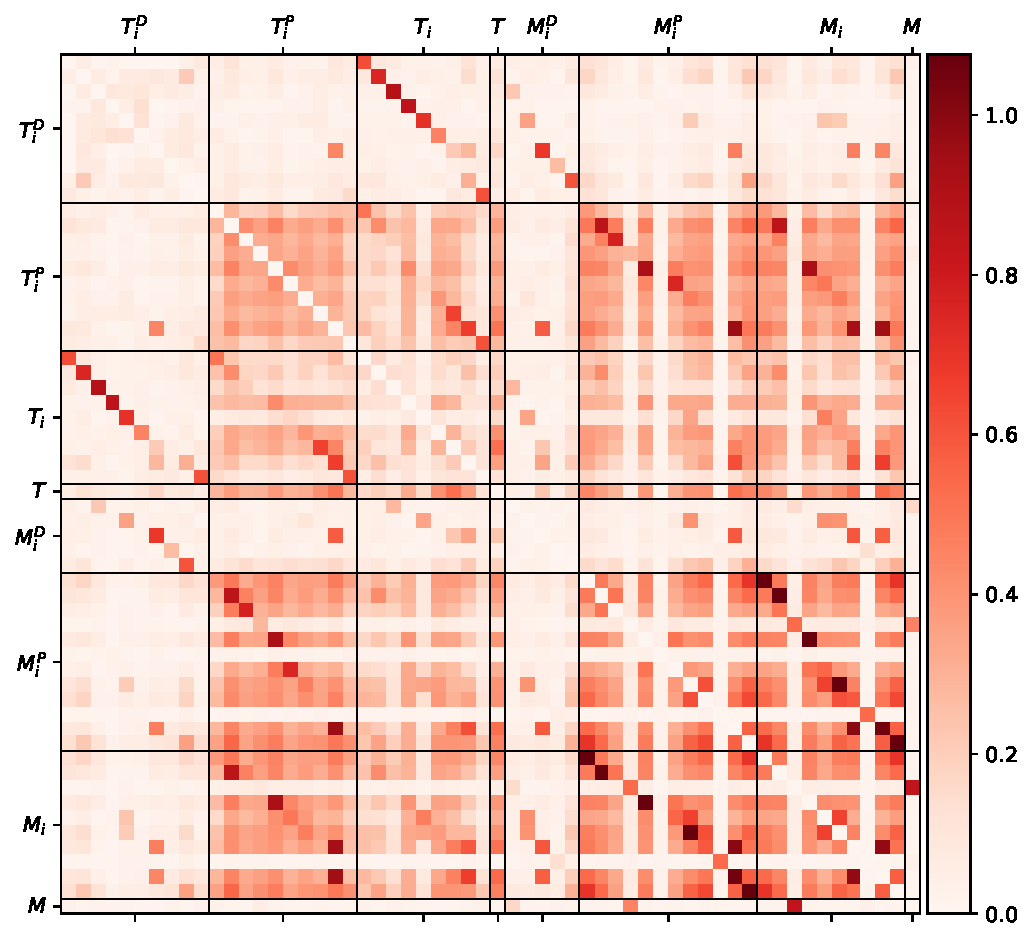
\includegraphics[width = 1\linewidth]{figures/Cycle data/G_obs complete - symmetric.pdf}
    \caption{$G_{obs}$ from pharmaceutical production data. Strong dependencies between variables and the related accumulated variables are observed.}
    \label{fig:Cycle data - G_obs all}
\end{figure}

\begin{figure}[ht]
    \centering
    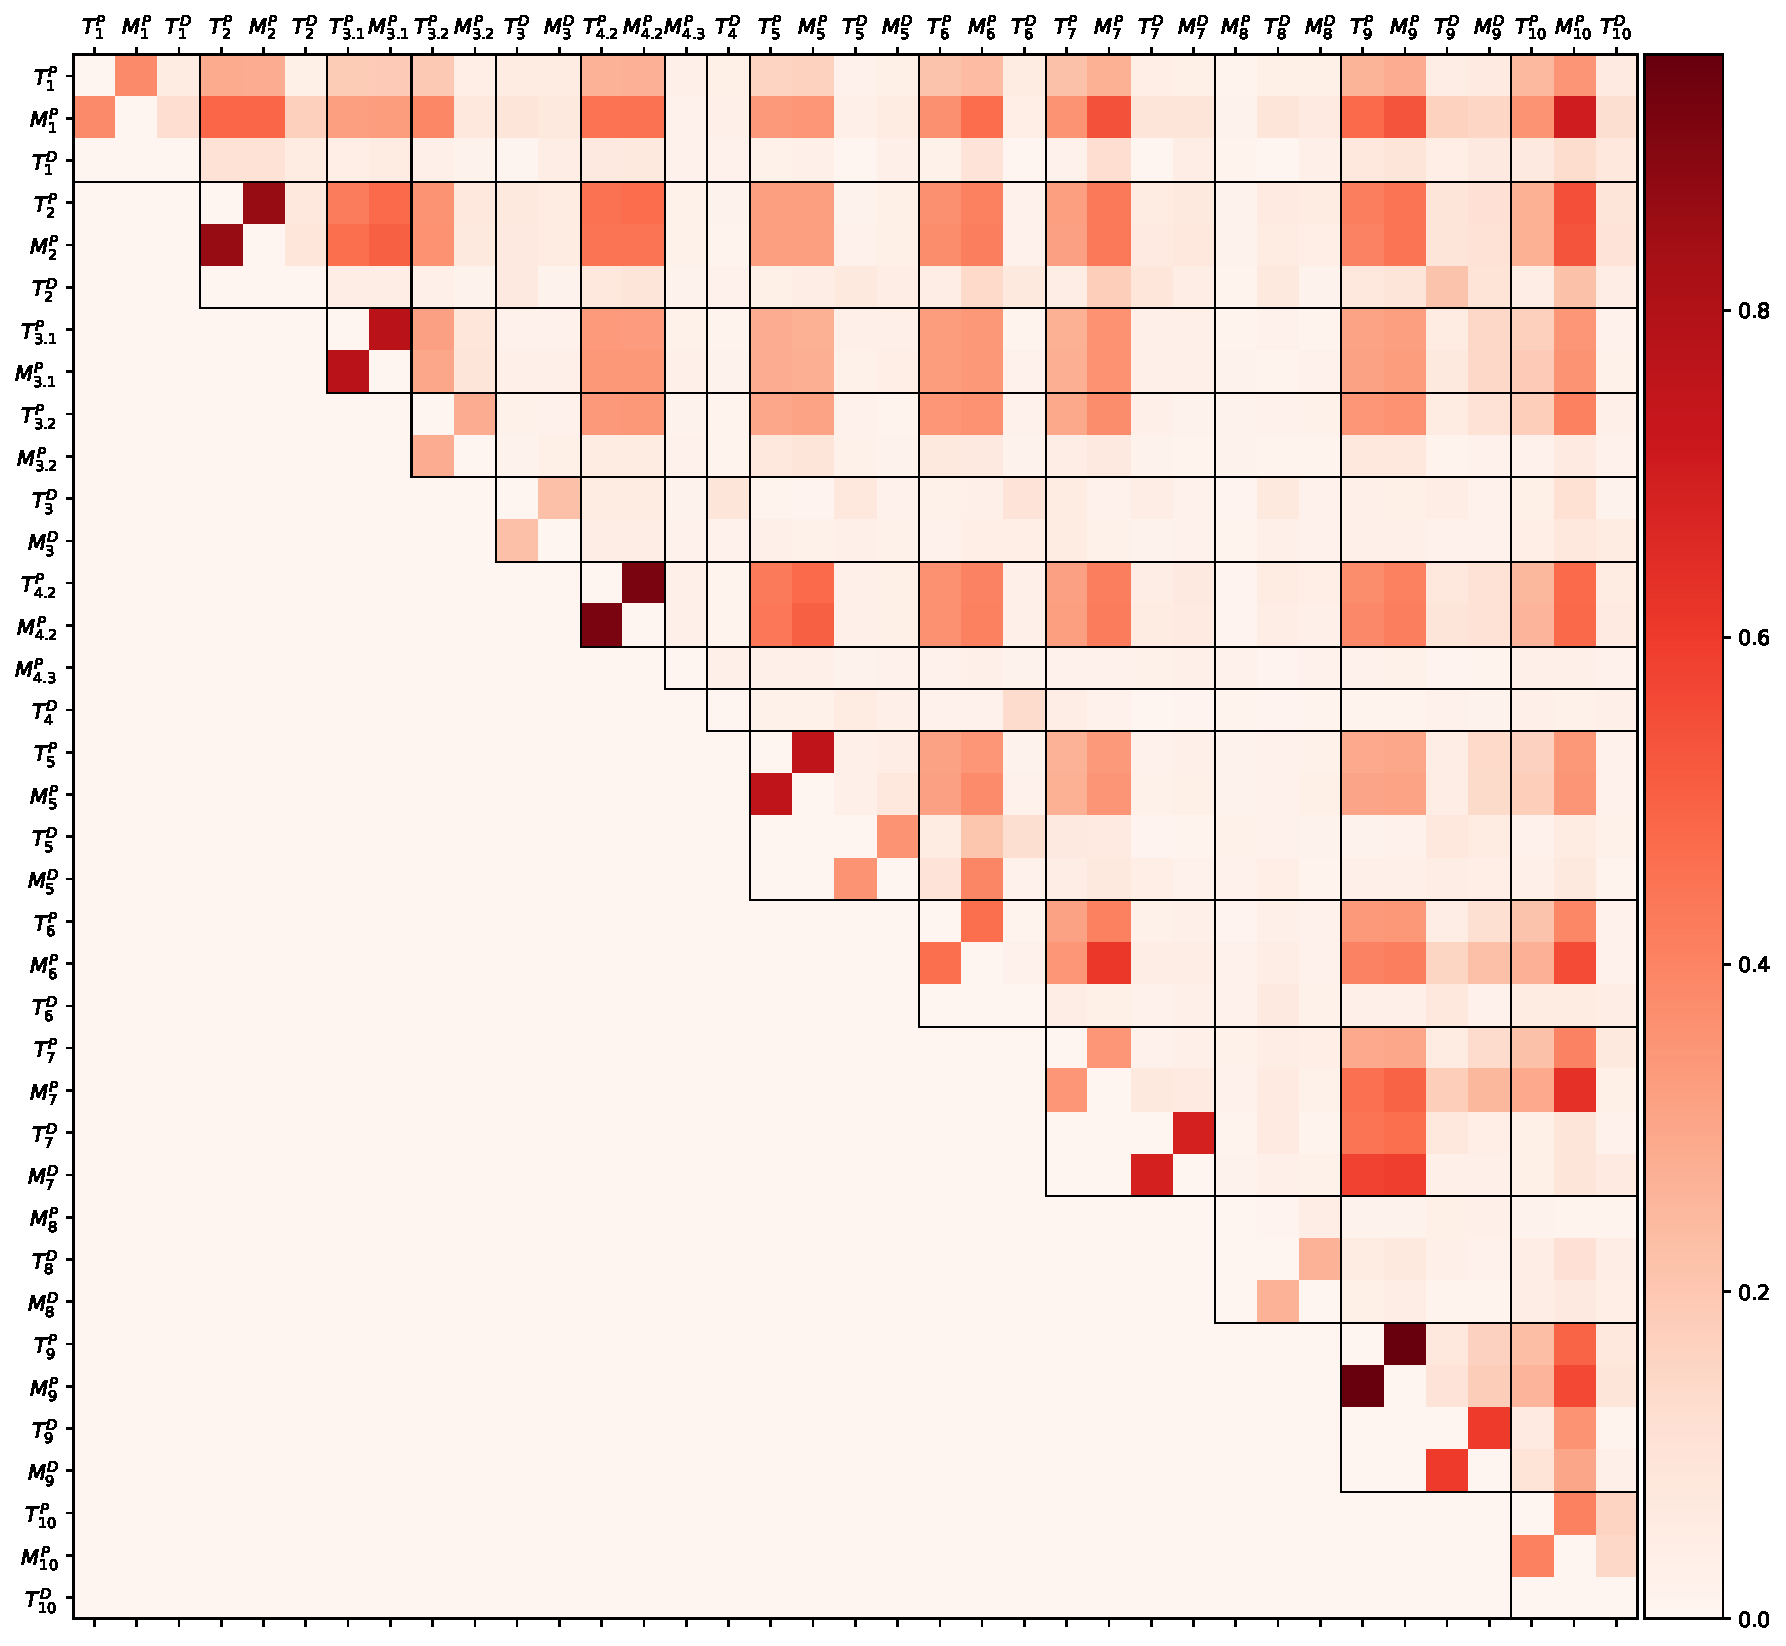
\includegraphics[width = \linewidth]{figures/Cycle data/G_obs times and levelchanges - semi-directed.pdf}
    \caption{$G_{obs}$ for both durations, delays and level changes for the simulated data from \cite{benchmark-model-to-generate-batch-process-data}. Labels related to the same process are divided by lines vertically and horizontally to easier observe what is related to what.}
    \label{fig:G_obs times and levelchanges - semi-directed}
\end{figure}

\end{document}